% !TEX root = mainthesis.texx
%Appendix 
\appendix
\renewcommand{\thechapter}{C}
\renewcommand{\chaptername}{Appendix}

\chapter{Full derivation of the Raman coupled $\xyz$ states}
\label{app:Rashba_derivation}

In this Appendix I derive the full time-dependent Hamiltonian describing the $\xyz$ states coupled by three Raman beams to produce Rashba type SOC (see Chapter~\ref{ch:Rashba}. It takes a bit of thinking to understand what the frequencies of the different Raman coupling terms correspond to in the RF rotating frame where the $\xyz$ states are defined. Hopefully this Appendix helps to clarify our specific choices for the laser geometry and polarization. 


Our system is based on the proposal described in~\cite{campbell_rashba_2016} to engineer a system with Rashba-like SOC. We consider $\Rb87$ atoms in the ground hyperfine $F=1$ manifold subject to a constant magnetic field $B_0\ez$ and an RF magnetic field $B_{\rm{RF}}\cos(\omrf t)\ex$ as in Chapter~\ref{ch:clock_states}. The system is described by the Hamiltonian
%
\begin{equation}
\hat H_{\rm{RF}} = \omega_0 \fz - \frac{\epsilon}{\hbar} (\fz^2-\mathbb{1})+2\Omrf\cos(\omrf t)\fx,
\label{Eq:H_RF}
\end{equation}
%
where $\omega_0 = g_F\mu_B B_0$ is the Larmor frequency, $\epsilon$ is a quadratic Zeeman\footnote{the quadratic dependence of $\epsilon$ on the applied bias field is not explicitly indicated on the symbol but is important to take into account to get the detuning just right} shift that breaks the degeneracy of the $\ket{m_F=-1}\leftrightarrow$ $\ket{m_F=0}$ and $\ket{m_F=1}\leftrightarrow$ $\ket{m_F=0}$ transitions, $\Omrf = g_F\mu_B B_{\rm{RF}} / 2$ is the RF coupling strength and $\mathbb{1}$ is the identity matrix. We transform the Hamiltonian into the  RF rotating frame using the unitary transformation $\hat U(t) = \exp(-i \omrf t \fz)$. The spin-1 operators under this transformation become
\begin{align}
\begin{split}
\fx  & \rightarrow \cos(\omrf t)\fx -\sin(\omrf t)\fy \\
     & = e^{i\omega_{\rm{RF}}t}\fp +e^{-i\omega_{\rm{RF}}t}\fm\\
\fy & \rightarrow \sin(\omrf t)\fx + \cos(\omrf t)\fy \\
     &=\frac{1}{i}(e^{i\omega_{\rm{RF}}t}\fp-e^{-i\omega_{\rm{RF}}t}\fm) \\
\fz & \rightarrow \fz.
\label{eq:rotation_transformations}
\end{split}
\end{align}
%
The unitary evolution in the rotating frame is described by the transformed Hamiltonian $\hat U^{\dagger}(t)(\hat H_{\rm{RF}} -i \hbar \partial_t)\hat U(t)$, which after neglecting terms that are oscillating with angular frequency $2\omrf$ is 

\begin{equation}
\hat H_{RWA}= \Delta \fz - \frac{\epsilon}{\hbar} (\fz^2-\mathbb{I}) + \Omrf \fx
\label{Eq:H_RWA}
\end{equation}
%
\begin{figure*}[!htb]
	\begin{center}
		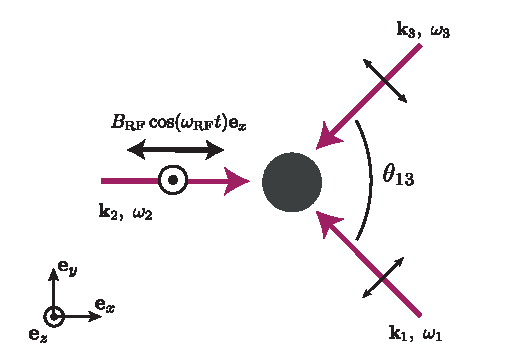
\includegraphics{Figures/AppendixC/Rashba_layout.pdf}
		\caption
		{Laser layout:  We use a strong RF field and three linearly polarized Raman beams propagating in the $xy$ plane couple the $\xyz$ states and engineer the Rashba Hamiltonian. 
		\label{fig:Rashba_layout}}
	\end{center}
\end{figure*}
%
The eigenstate of Equation~\ref{Eq:H_RWA} are the $\xyz$ states described in Chapter~\ref{ch:clock_states}. Now we apply three Raman beams as shown in Figure~\ref{fig:Rashba_layout}. This configuration differs from the one proposed in~\cite{campbell_rashba_2016} for technical reasons as we wanted all the Raman recoil vectors to lie within the imaging plane of the experiment which corresponds to the $xy$ plane. 

The electric field at the atoms in the lab (not rotating) frame is
%
\begin{equation}
\mathbf{E}(x, t)=\sum_{i=1}^{3}E_i\mathbf{e}_i e^{i(\mathbf{k}_i\cdot\mathbf{x}-\omega_i t)},
\label{eq:Raman_basic}
\end{equation}
%
where $E_i$ is the field amplitude, $\omega_i$ is the angular frequency, $\k_i$ is the wave vector and $\mathbf{e}_i$ is the polarization of each of the beams. In order to have the right coupling matrix elements to cyclically couple all three states in a ring-like coupling as described in~\cite{campbell_realistic_2011} we need a Hamiltonian of the form

\begin{equation}
	\hat{H}_{\rm{SOC}}=(\Omega_x, \Omega_y, \Omega_z)\cdot \hat{\mathbf{F}}
\end{equation}
%
(see Section~\ref{sec:xyz_matrix_elements}). This is possible if we choose two Raman beams to have in plane polarization and one vertically polarized beam:
%
\begin{align}
\begin{split}
\mathbf{e}_1&=\frac{(k_{1y}, -k_{1x}, 0)}{\vert\vert \mathbf k_1 \vert\vert^2}, \\
\mathbf{e}_2&=(0, 0, 1), \\
\mathbf{e}_3&=\frac{(k_{3y}, -k_{3x}, 0)}{\vert\vert \mathbf k_3 \vert\vert^2}, \\
\label{eq:polarization}
\end{split}
\end{align}
%

The Raman coupling strength is proportional to the vector polarizability (see Section~\ref{sec:vector_polarizability}) and the Hamiltonian describing the atom-light coupling is
%
\begin{equation}
\hat{H}_R=(iu_v\mathbf E\times\mathbf E^*)\cdot\hat F,
\label{eq:vector_stark}
\end{equation}
%
where $u_v$ is the vector polarizability. The expression for the cross product of the electric field at the atoms is quite messy, lets rewrite it in a more convenient way:

\begin{align}
\begin{split}
\mathbf E\times\mathbf E^* &= (E_1^* \e_1 e^{-i(\mathbf k_1\cdot \mathbf x -\omega_1 t)}
					       +E_2^* \e_2 e^{-i(\mathbf k_2\cdot \mathbf x -\omega_2 t)} 
					       +E_3^* \e_3 e^{-i(\mathbf k_3\cdot \mathbf x -\omega_3 t)})
					       \times c.c \\
					  & = E_1^*E_2(\e_1\times \e_2)e^{i[(\k_2-\k_1)\cdot\x-(\omega_2-\omega_1)t]}
					      + E_1^*E_3(\e_1\times \e_3)e^{i[(\k_3-\k_1)\cdot\x-(\omega_3-\omega_1)t]} \\
					  & + E_2^*E_1(\e_2\times \e_1)e^{i[(\k_1-\k_2)\cdot\x-(\omega_1-\omega_2)t]}	 
					     + E_2^*E_3(\e_2\times \e_3)e^{i[(\k_3-\k_2)\cdot\x-(\omega_3-\omega_2)t]} \\
					  & + E_3^*E_1(\e_3\times \e_1)e^{i[(\k_1-\k_3)\cdot\x-(\omega_1-\omega_3)t]}
					     +  E_3^*E_2(\e_3\times \e_2)e^{i[(\k_2-\k_3)\cdot\x-(\omega_2-\omega_3)t]} \\
					  &=2i\big[ (\e_1\times\e_2) \text{Im}
					  	\{E_1^*E_2\ e^{i(\k_{21}\cdot \x - \omega_{21} t)}\} \\
					& +(\e_1\times\e_3) \text{Im}\{E_1^*E_3\ e^{i(\k_{32}\cdot \x - \omega_{32} t)}\} \\
					& +(\e_2\times\e_3) \text{Im}\{E_2^*E_3\ e^{i(\k_{32}\cdot \x - \omega_{32} t)}\} \big]
\end{split}
\end{align}
%
and using the definition of the polarization vectors (Equation~\ref{eq:polarization})
%
\begin{align}
\begin{split}
\e_1\times \e_2 &= \frac{(-k_{1x}, -k_{1y}, 0)}{\vert\vert \k_1\vert\vert^2} = -\hat\k_1 \\
\e_1\times \e_3 &= \frac{(0, 0, -k_{1y}k_{3x}+k_{3y}k_{1x})}{\vert\vert \k_1\vert\vert^2\vert\vert \k_3\vert\vert^2} = \ez\sin\theta_{13}\\
\e_2\times\e_3 &= \frac{(k_{3x}, k_{3y}, 0)}{\vert\vert \k_3\vert\vert^2} = \hat\k_3,
\end{split}
\end{align}
%
we obtain the the desired Hamiltonian describing the atom light interaction
\begin{align}
\begin{split}
iu_v\mathbf E^* \times\mathbf E \cdot\mathbf{\hat{F}}&= -2u_v\big[-\hat\k_1\text{Im}\{12\}+\ez\sin\theta_{13}\text{Im}\{13\}+\hat\k_3\text{Im}\{23\}\big] \cdot \hat{\mathbf{F}}\\
&=(\Omega_x, \Omega_y, \Omega_z)\cdot \hat{\mathbf{F}},
\label{eq:full_Raman}
\end{split}
\end{align}
%
where
\begin{align}
\begin{split}
\Omega_x &=\frac{k_{1x}}{\vert\vert\k_1\vert\vert}\text{Im}\{\Omega_{12}e^{i(\k_{21}\cdot\x-\omega_{21}t)}\}
		+\frac{k_{3x}}{\vert\vert\k_3\vert\vert}\text{Im}\{\Omega_{23}e^{i(\k_{32}\cdot\x-\omega_{32}t)}\}\\
\Omega_y &=\frac{k_{1y}}{\vert\vert\k_1\vert\vert}\text{Im}\{\Omega_{12}e^{i(\k_{21}\cdot\x-\omega_{21}t)}\}
		+\frac{k_{3y}}{\vert\vert\k_3\vert\vert}\text{Im}\{\Omega_{23}e^{i(\k_{32}\cdot\x-\omega_{32}t)}\}\\
\Omega_z &=\text{Im} \{\Omega_{13}e^{i(\k_{31}\cdot\x-\omega_{31}t)}\},
\end{split}
\end{align} 
and
\begin{align}
\begin{split}
\Omega_{12}&=2u_vE_1^*E_2 \\
\Omega_{13}&=-2u_vE_1^*E_3\sin\theta_{13}\\
\Omega_{23}&=-2u_vE_2^*E_3.
\end{split}
\end{align}


Now we need to transform Eq.~\ref{eq:full_Raman} into the rotating frame, this is where things start getting fun. The `slow' or `fast' nature of a given term depends on the specific choice of frequencies on each Raman beam which should be such that the frequency differences $\omega_{ij}$ are resonant with dressed state transitions in the rotating frame as shown in Figure~\ref{fig:Rashba_frequencies}a. 

I showed in Equation~\ref{eq:rotation_transformations} that in the rotating frame the $\fx$ and $\fy$ operators get additional factors of $\exp(\pm i\omega_{\rm{RF}})$ while $\fz$ remains unchanged. We must therefore have the frequencies of beams giving rise to $\fx$ and $\fy$ coupling to differ in frequency by an additional $\omrf$ and the beams that give the $\fz$ coupling to be close in frequency. The two possible ways of doing so are shown in Figure~\ref{fig:Rashba_frequencies}b and they determine weather $\omega_{21}$ and $\omega_{31}$ are positive or negative.

\begin{figure*}[!htb]
	\begin{center}
		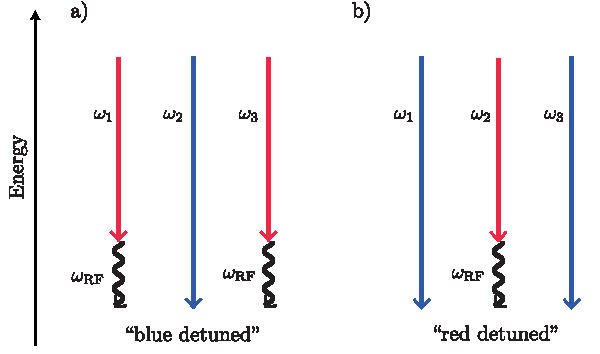
\includegraphics{Figures/AppendixC/laser_frequencies.pdf}
		\caption[Raman coupling of the $\xyz$ states]
		{{\bf a} The choice of laser frequencies should be such that in the frame rotating with frequency $\omrf$ we get resonant Raman coupling of the $\xyz$ states. {\bf b.} Possible laser frequency configurations: {\bf{i)}} Blue detuned configuration: There are 2 frequencies smaller by about $\omega_{\rm{RF}}$ and one larger frequency. {\bf{ii)}} The red detuned configuration: there are 2 frequencies that are larger by about $\omega_{\rm{RF}}$ and one smaller frequency. 
		\label{fig:Rashba_frequencies}}
	\end{center}
\end{figure*}

%
Lets look at the firs term of the $\Omega_x\fx$ coupling to get an idea of how the RWA will work here:
\begin{align}
\begin{split}
\Omega_x ^{(1)}\fx &\rightarrow\frac{1}{4i}\frac{k_{1x}}{\vert\vert\k_1\vert\vert}
\left(\Omega_{12}e^{i(\k_{21}\cdot\x-\omega_{21})t} - \Omega_{12}^*e^{-i(\k_{21}\cdot\x-\omega_{21}t)}\right)\left(e^{i\omega_{\rm{RF}}t}\fp +e^{-i\omega_{\rm{RF}}t}\fm\right) \\
& \approx \frac{1}{4i}\frac{k_{1x}}{\vert\vert\k_1\vert\vert}
\left(\Omega_{12}e^{i(\k_{21}\cdot\x-(\omega_{21}\mp\omega_{\rm{RF}})t)}\hat{F}_{\pm} 
- \Omega_{12}^*e^{-i(\k_{21}\cdot\x-(\omega_{21}\mp \omega_{\rm{RF}})t)}\hat{F}_{\mp}\right) \\
% & = \frac{1}{4i}\frac{k_{1x}}{\vert\vert\k_1\vert\vert}
% \left(\Omega_{12}e^{i(\k_{21}\cdot\x-(\omega_{21}\mp\omega_{\rm{RF}})t)}-c.c.\right)\fx
% \pm i\left(\Omega_{12}e^{i(\k_{21}\cdot\x-(\omega_{21}\mp\omega_{\rm{RF}})t)}+c.c.\right)\fy \\
& = \frac{1}{2}\frac{k_{1x}}{\vert\vert\k_1\vert\vert}\vert\Omega_{12}\vert\Big(\sin[\k_{21}\cdot\x-(\omega_{21}\mp\omega_{\rm{RF}})t+\phi_{12}]\fx \\
&\pm\cos[\k_{21}\cdot\x-(\omega_{21}\mp\omega_{\rm{RF}})t+\phi_{12}]\fy\Big).
\end{split}
\end{align} 
%
Here the upper sign corresponds to the $\omega_{21}>0$ case (blue detuned) and the lower sign to $\omega_{21}<0$ (red detuned) and I performed a RWA approximation in the second line by neglecting the terms oscillating with frequency close to $2\omrf$. Similarly, the second therm of $\Omega_x\fx$ is
\begin{align}
\begin{split}
\Omega_x ^{(2)}\fx &\rightarrow\frac{1}{4i}\frac{k_{3x}}{\vert\vert\k_3\vert\vert}
\left(\Omega_{23}e^{i(\k_{32}\cdot\x-\omega_{32})t} - \Omega_{23}^*e^{-i(\k_{32}\cdot\x-\omega_{32}t)}\right)\left(e^{i\omega_{\rm{RF}}t}\fp +e^{-i\omega_{\rm{RF}}t}\fm\right) \\
& \approx  \frac{1}{2}\frac{k_{3x}}{\vert\vert\k_3\vert\vert}\vert\Omega_{23}\vert
\Big(\sin[\k_{32}\cdot\x-(\omega_{32}\mp\omega_{\rm{RF}})t+\phi_{23}]\fx \\
&\pm\cos[\k_{32}\cdot\x-(\omega_{32}\mp\omega_{\rm{RF}})t+\phi_{23}]\fy\Big)
\end{split}
\end{align}
%
where I used the same sign convention as before. It is important to keep in mind that if $\omega_{21}$ is positive then $\omega_{32}$ must be negative and vice versa. 
%
Lets keep cranking the algebra!
\begin{align}
\begin{split}
\Omega_y^{(1)}\fy& \rightarrow -\frac{1}{4}\frac{k_{1y}}{\vert\vert\k_1\vert\vert}
\left(\Omega_{12}e^{i(\k_{21}\cdot\x-\omega_{21}t} - \Omega_{12}^*e^{-i(\k_{21}\cdot\x-\omega_{21}t)}\right)
\left(e^{i\omega_{\rm{RF}}t}\fp-e^{-i\omega_{\rm{RF}}t}\fm\right) \\
& \approx \mp\frac{1}{4}\frac{k_{1y}}{\vert\vert\k_1\vert\vert} 
\left(\Omega_{12}e^{i(\k_{21}\cdot\x-(\omega_{21}\mp\omega_{\rm{RF}})t)}\hat{F}_{\pm} 
+ \Omega_{12}^*e^{-i(\k_{21}\cdot\x-(\omega_{21}\mp \omega_{\rm{RF}})t)}\hat{F}_{\mp}\right) \\
% &=\mp\frac{1}{4}\frac{k_{1y}}{\vert\vert\k_1\vert\vert} 
% \left(\left(\Omega_{12}e^{i(\k_{21}\cdot\x-(\omega_{21}\mp\omega_{\rm{RF}})t)} + c.c.\right)\fx 
% + i\left(\Omega_{12}e^{i(\k_{21}\cdot\x-(\omega_{21}\mp\omega_{\rm{RF}})t)} - c.c.\right)\fy \right) \\
&= \mp\frac{1}{2}\frac{k_{1y}}{\vert\vert\k_1\vert\vert} 
\vert\Omega_{12}\vert\Big(\cos[\k_{21}\cdot\x-(\omega_{21}\mp\omega_{\rm{RF}})t+\phi_{12}]\fx \\
&-\sin[\k_{21}\cdot\x-(\omega_{21}\mp\omega_{\rm{RF}})t+\phi_{12}]\fy\Big),
\end{split}
\end{align}
%

\begin{align}
\begin{split}
\Omega_y^{(2)}\fy& \rightarrow -\frac{1}{4}\frac{k_{3y}}{\vert\vert\k_3\vert\vert}
\left(\Omega_{23}e^{i(\k_{32}\cdot\x-\omega_{32}t} - \Omega_{23}^*e^{-i(\k_{32}\cdot\x-\omega_{32}t)}\right)
\left(e^{i\omega_{\rm{RF}}t}\fp-e^{-i\omega_{\rm{RF}}t}\fm\right) \\
&\approx \mp\frac{1}{2}\frac{k_{3y}}{\vert\vert\k_3\vert\vert} 
\vert\Omega_{23}\vert\Big(\cos[\k_{32}\cdot\x-(\omega_{32}\mp\omega_{\rm{RF}})t+\phi_{23}]\fx \\
&-\sin[\k_{32}\cdot\x-(\omega_{32}\mp\omega_{\rm{RF}})t+\phi_{23}]\fy\Big).
\end{split}
\end{align}
%
The complete Hamiltonian in the rotating frame after doing the rotating wave approximation is then
%
\begin{align}
\begin{split}
\hat{H}= \frac{1}{2}\frac{\vert\Omega_{12}\vert}{\vert\vert\k_1\vert\vert}
\Bigg(&\Big(k_{1x}\sin[\k_{21}\cdot\x-(\omega_{21}\mp\omega_{\rm{RF}})t+\phi_{12}]
\pm k_{1y}\cos[\k_{21}\cdot\x-(\omega_{21}\pm\omega_{\rm{RF}})t+\phi_{12}]\Big)\fx \\
+ &\Big(\pm k_{1x}\cos[\k_{21}\cdot\x-(\omega_{21}\mp\omega_{\rm{RF}})t+\phi_{12}]
\mp k_{1y}\sin[\k_{21}\cdot\x-(\omega_{21}\pm\omega_{\rm{RF}})t+\phi_{12}]\Big)\fy\Bigg) \\
\frac{1}{2}\frac{\vert\Omega_{23}\vert}{\vert\vert\k_3\vert\vert}
\Bigg(&\Big(k_{3x}\sin[\k_{32}\cdot\x-(\omega_{32}\mp\omega_{\rm{RF}})t+\phi_{23}]
\pm k_{3y}\cos[\k_{32}\cdot\x-(\omega_{32}\pm\omega_{\rm{RF}})t+\phi_{23}]\Big)\fx \\
+ &\Big(\pm k_{3x}\cos[\k_{32}\cdot\x-(\omega_{32}\mp\omega_{\rm{RF}})t+\phi_{23}]
\mp k_{3y}\sin[\k_{32}\cdot\x-(\omega_{32}\pm\omega_{\rm{RF}})t+\phi_{23}]\Big)\fy \Bigg)\\
+&\vert\Omega_{13}\vert\sin(\k_{31}\cdot\x - \omega_{31}t+\phi_{13})\fz
\label{eq:complete_Rashba}
\end{split}
\end{align}
%

In order to go from this rather complicated looking Hamiltonian to the effective time independent Hamiltonian used in Chapter~\ref{ch:Rashba} we need to take two steps: first the off resonant coupling terms need to be neglected. This can be more or less safely done since they will be detuned by something on the order of tens to hundreds of kHz. Second we need to go into a second transformed frame using the unitary transformation
%
\begin{equation}
\hat{U}=\sum_{i\in\{xyz\}}e^{i(\k_i\cdot\x-\omega_it)}	
\end{equation}
%
and eliminate the terms that are proportional to $\exp(i\omega_{ij}t)$. The neglected terms of the Hamiltonian in Equation~\ref{eq:complete_Rashba} have the effect of slightly shifting the eigenenergies of the effective Hamiltonian from Equation~\ref{Eq:Rashba_atoms}. We interpret this shifts in energy as coming from new effective Raman coupling strengths that slightly differ from our calibrations performed by measuring the Rabi frequencies of individual pairs of Raman beams. 


% \begin{figure*}[htb]
% \begin{center}
% 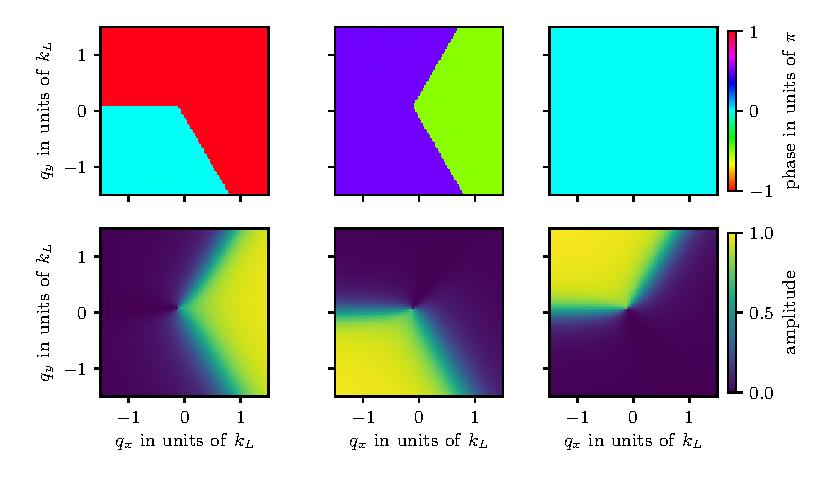
\includegraphics[]{Figures/Chapter8/topological_eigenvecs.pdf}
% \caption{{\bfseries a} Probabilities as a function of quasimomentum for the three output ports of the interferometer at $t_{\rm free}=\unit[160]{\mu s}$ {\bfseries b} Probabilities as a function of free evolution time $t_{\mathrm{free}}$ for an input state with quasimomentum $(q_1, q_2)=(0.55,-0.92)\,k_{\rm L}$ indicated by the blue star on {\bfseries a} and in the topological ground branch ($n=1$)}
% \label{fig:topological_eigenvecs}
% \end{center}
% \end{figure*}

% \begin{figure*}[htb]
% \begin{center}
% 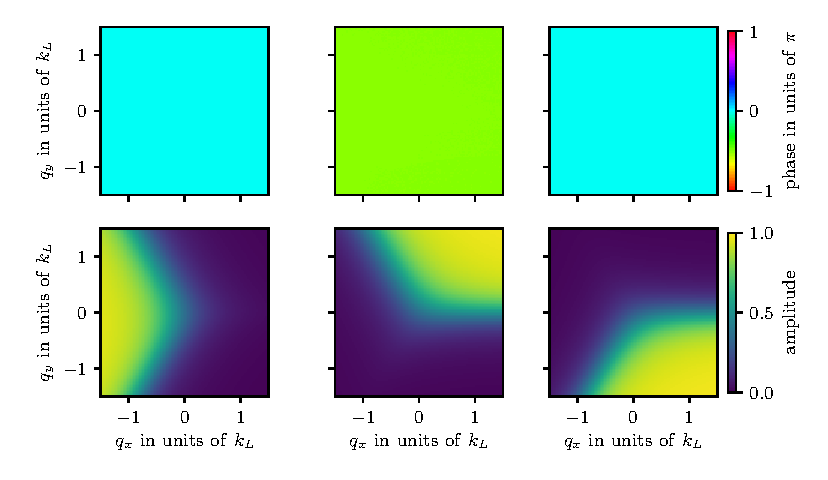
\includegraphics[]{Figures/Chapter8/nontopological_eigenvecs.pdf}
% \caption{{\bfseries a} Probabilities as a function of quasimomentum for the three output ports of the interferometer at $t_{\rm free}=\unit[160]{\mu s}$ {\bfseries b} Probabilities as a function of free evolution time $t_{\mathrm{free}}$ for an input state with quasimomentum $(q_1, q_2)=(0.55,-0.92)\,k_{\rm L}$ indicated by the blue star on {\bfseries a} and in the topological ground branch ($n=1$)}
% \label{fig:nontopological_eigenvecs}
% \end{center}
% \end{figure*}
